% NeSy 2027 submission
\documentclass[final]{nesy2027}

\usepackage{booktabs}
\usepackage{listings}
\usepackage{xcolor}
\usepackage{amsmath}
\usepackage{hyperref}
\usepackage{natbib}
\usepackage{markdown}

% Style for DSL code listings
\lstdefinestyle{dslstyle}{
  basicstyle=\ttfamily\small,
  backgroundcolor=\color{gray!10},
  frame=single,
  framerule=0.4pt,
  breaklines=true,
  columns=flexible,
}

\title[Neural DSL Navigation]{Learning Latent Program Spaces through Neural DSL Navigation%
  \titletag{\thanks{Code available at https://github.com/Julien-Livet/aicpp}}}

\clearauthor{%
  \Name{Julien Livet} \Email{julien.livet@free.fr}\\
  \addr{Independent Researcher}
}

\begin{document}

\maketitle

% ─────────────────────────────────────────────────────────────────────────────
\begin{abstract}
This paper presents an exploratory neuro-symbolic approach for learning a
latent representation of programs expressed in a Domain-Specific Language (DSL)
inspired by ARC-style grid transformations.
The system combines Graph Neural Networks (GNNs), Convolutional Neural Networks
(CNNs), and Transformers within a unified architecture trained with an iterative
cost-guided objective.
Preliminary empirical observations indicate that structured neighbourhoods emerge
\emph{spontaneously} in the embedding space, with programs clustering by
semantic function (rotations, mirrors, reductions, concatenations).
Furthermore, the model exhibits non-trivial conceptual transitions during program
search, including the formation of anchors and star-shaped exploration patterns.
These results suggest that the proposed method offers a promising direction for
explainable, data-efficient neuro-symbolic program synthesis.
\end{abstract}

% ─────────────────────────────────────────────────────────────────────────────
\section{Introduction}
\label{sec:intro}

The field of Neuro-Symbolic Artificial Intelligence has experienced rapid
growth, with research efforts concentrated in learning and inference (63\%),
logic and reasoning (35\%), and knowledge representation (44\%)
\citep{colelough2025neurosymbolic}.
However, significant gaps remain in \textbf{explainability} (28\%) and
\textbf{meta-cognition} (5\%) -- areas that are critical for deploying AI
systems in high-stakes domains such as industrial automation, healthcare, and
formal verification.

Program synthesis -- the automatic construction of programs from specifications
-- remains a challenging task due to the combinatorial explosion of the search
space.
Pure neural approaches lack interpretability, while pure symbolic methods
struggle with scalability and noise tolerance.

This paper investigates a hybrid approach where: (i)~a \textbf{DSL} provides a
structured symbolic vocabulary; (ii)~a \textbf{neural architecture}
(GNN + CNN + Transformer) learns a continuous latent space of programs;
and (iii)~an \textbf{iterative cost-guided search} navigates this space using a
multi-component heuristic.

We demonstrate that this architecture leads to the \textbf{spontaneous emergence
of a semantic map} of the program space, where programs with similar effects
cluster together -- without any explicit semantic supervision.

% ─────────────────────────────────────────────────────────────────────────────
\section{Related Work}
\label{sec:related}

\paragraph{Neuro-Symbolic AI.}
Recent systematic reviews \citep{colelough2025neurosymbolic} highlight a growing
interest in integrating symbolic reasoning with deep learning.
Approaches range from logically constrained neural networks
\citep{mao2019neuro} to graph-based knowledge representation
\citep{schlichtkrull2018modeling}.
However, most works focus on classification or reasoning tasks, not on program
synthesis.

\paragraph{Program Synthesis.}
Classical approaches use deductive synthesis \citep{gulwani2011automating},
while modern methods leverage large language models (LLMs) for code generation
\citep{chen2021evaluating}.
LLMs lack explicit program structure and are difficult to constrain.
DreamCoder \citep{ellis2021dreamcoder} introduced wake-sleep library learning
for program induction from examples, and STITCH \citep{bowers2023stitch} further
refined top-down abstraction in DSL spaces.
Our approach complements these by learning a \emph{continuous} latent map of the
program space rather than a discrete library.

\paragraph{Latent Program Spaces.}
Several works have explored continuous representations of programs through
variational autoencoders \citep{bunel2017learning} or by training transformers on
program traces \citep{zaremba2015learning}.
However, these often produce unstructured latent spaces.
Our work shows that structured semantic maps can emerge when using a typed DSL
combined with a multi-component cost function.

\paragraph{ARC and ARC-AGI.}
The Abstraction and Reasoning Corpus (ARC) \citep{chollet2019measure} is a
benchmark for measuring general intelligence.
Neuro-symbolic approaches to ARC remain rare, with most top performers relying
on combinatorial search \citep{hodel2024arc}.
This work positions itself within this niche.

% ─────────────────────────────────────────────────────────────────────────────
\section{The C++ Domain-Specific Language}
\label{sec:dsl}

The proposed approach relies on a domain-specific language (DSL) implemented
in C++. The DSL defines the executable vocabulary available to the program
synthesis system. Rather than generating unrestricted source code, the model
therefore operates over a constrained space of semantically meaningful
programs.

\subsection{DSL Design Principles}
\label{subsec:dsl-design}

The DSL is designed around three main principles.

First, each primitive represents a meaningful transformation in the target
domain. The vocabulary is therefore considerably smaller than a general
purpose programming language.

Second, primitives are strongly typed according to their input and output
domains. This allows syntactically invalid compositions to be rejected during
program construction.

Third, DSL programs are directly executable by the C++ engine. A generated
program can consequently be evaluated against the training examples without
requiring an additional interpretation or compilation step.

These properties constrain the search space while preserving an explicit
representation of the transformations performed by a synthesized program.

\subsection{Typed Primitives}
\label{subsec:dsl-types}

Each DSL primitive is associated with a fixed signature describing its input
and output types. For example, an image transformation may be represented as

\begin{verbatim}
Image mirror(Image input)
\end{verbatim}

while a parameterized transformation can be represented as

\begin{verbatim}
Image upscale(Image input, Integer factor)
\end{verbatim}

The type system consequently constrains the combinations of primitives that
can be considered during synthesis. This is particularly important when the
program space contains primitives with heterogeneous signatures.

In the implementation, primitive signatures are exposed to the synthesis
engine through the C++ representation of the DSL. The model does not have to
learn these typing constraints from the data alone: they are explicitly
encoded in the program-generation mechanism.

\subsection{Program Representation}
\label{subsec:dsl-program-representation}

A DSL program is represented as a composition of primitive applications.
For example, a transformation can be expressed as

\begin{verbatim}
hconcat(vmirror(I), cmirror(I))
\end{verbatim}

where $I$ denotes the input grid.

Nested expressions naturally form a tree structure. This representation is
used both for program generation and for constructing the graph representation
provided to the neural model.

The tree representation also makes the synthesized programs directly
inspectable by a human observer. Unlike a latent representation in which the
reasoning process is not directly observable, a generated DSL program
explicitly exposes the sequence of transformations selected by the system.

\subsection{Executable Semantics}
\label{subsec:dsl-execution}

The C++ engine provides the operational semantics of the DSL. Given a valid
program and an input grid, the engine recursively evaluates the corresponding
expression tree and produces an output grid.

The same execution mechanism is used during program search to evaluate
candidate programs against the training examples. A candidate program can
therefore be assigned a cost according to its discrepancy with the expected
outputs.

Let $P$ denote a synthesized program and let
$(X_i,Y_i)_{i=1}^{N}$ denote the training pairs. The program cost can
abstractly be written as

\[
C(P) =
\sum_{i=1}^{N}
D\left(P(X_i),Y_i\right),
\]

where $D$ is the discrepancy measure implemented by the evaluation engine.

A value of $C(P)=0$ indicates that the synthesized program reproduces all
training outputs exactly.

\subsection{DSL-Constrained Program Search}
\label{subsec:dsl-search}

The DSL induces a structured program space

\[
\mathcal{P}_{\mathrm{DSL}}
=
\left\{
P \mid P \text{ is a well-typed composition of DSL primitives}
\right\}.
\]

Program synthesis is consequently performed over
$\mathcal{P}_{\mathrm{DSL}}$ rather than over arbitrary programs.

For a maximum synthesis depth $d$, the search space can be viewed as the
subset

\[
\mathcal{P}_{\mathrm{DSL}}^{(\leq d)}
=
\left\{
P\in\mathcal{P}_{\mathrm{DSL}}
\mid
\operatorname{depth}(P)\leq d
\right\}.
\]

This depth constraint provides a direct mechanism for controlling the
computational complexity of synthesis.

The search engine evaluates candidate programs and retains programs that
improve the current cost. Consequently, the search trajectory provides an
explicit record of the successive hypotheses considered by the system.

\subsection{Integration with the Neural Model}
\label{subsec:dsl-neural-integration}

The DSL is not used solely as an execution language. It also constitutes the
interface between neural prediction and symbolic program synthesis.

The neural model predicts DSL tokens and program structures, while the
symbolic engine validates and executes the resulting programs. Candidate
programs can subsequently be represented as program graphs and combined with
their observed execution costs before being provided to the model.

This creates a feedback loop between the neural and symbolic components:

\begin{enumerate}
    \item the neural model proposes a DSL program;
    \item the symbolic engine validates and executes the program;
    \item the resulting program is evaluated against the training examples;
    \item the execution cost provides feedback about the quality of the
          candidate;
    \item the resulting information is incorporated into the subsequent
          program-generation process.
\end{enumerate}

The architecture therefore combines learned program generation with
explicit symbolic execution.

\subsection{Interpretability of Synthesized Programs}
\label{subsec:dsl-interpretability}

An important consequence of the DSL representation is that successful or
partially successful hypotheses remain expressed as executable symbolic
programs.

For example, the search process can produce expressions such as

\begin{verbatim}
trim(trim(I))
\end{verbatim}

or

\begin{verbatim}
upscale(dedupe(I), TEN).
\end{verbatim}

Such expressions directly expose the transformations selected by the system.
They can therefore be inspected, executed independently, compared with
alternative hypotheses, and used to analyse the behaviour of the synthesis
process.

This property is particularly relevant to ARC-like tasks, where understanding
the transformation applied to an input grid is an important part of analysing
a solution.

\subsection{Domain Adaptability}
\label{subsec:dsl-adaptability}

The DSL is intended to separate the general synthesis mechanism from the
domain-specific vocabulary.

Changing the target domain primarily requires defining a new set of typed
primitives and their executable semantics. The neural and symbolic synthesis
components can then operate over this new vocabulary.

This design suggests that the same general architecture could potentially be
applied to domains other than grid transformations, provided that an
appropriate DSL can be defined.

% ─────────────────────────────────────────────────────────────────────────────
\section{Method}
\label{sec:method}

\subsection{Domain-Specific Language}
\label{sec:method-dsl}

We use a typed DSL derived from the Hodel DSL for ARC
\citep{hodel2024arc}, containing primitives such as rotations
(\texttt{rot90}, \texttt{rot180}, \texttt{rot270}), mirrors
(\texttt{hmirror}, \texttt{vmirror}, \texttt{cmirror}, \texttt{dmirror}),
reductions (\texttt{tophalf}, \texttt{bottomhalf}, \texttt{lefthalf},
\texttt{righthalf}), concatenations (\texttt{hconcat}, \texttt{vconcat}),
rescaling (\texttt{upscale}, \texttt{downscale}, \texttt{vupscale}), and value
transformations (\texttt{replace}, \texttt{switch}, \texttt{compress},
\texttt{trim}).

All programs are typed and must satisfy syntactic constraints enforced by a
\texttt{TreeState} mask: at each decoding step, only tokens whose type is
compatible with the current position in the Abstract Syntax Tree (AST) are
allowed. This guarantees that every generated program is syntactically valid by
construction.

\subsection{Architecture}
\label{sec:arch}

The model consists of three encoders and one constrained decoder, illustrated
schematically in Fig.~\ref{fig:arch}.

\textbf{ARC Grid Encoder (CNN).}
Each pair $(I_{\mathrm{in}}, I_{\mathrm{out}})$ is encoded by a four-layer CNN
(64$\to$64$\to$128$\to$128 channels, kernel size $3\times3$, padding 1) with
attention pooling over $N$ pairs.
The input tensor concatenates one-hot colour channels, the pixel-wise difference
map, and a validity mask.
Output: $z_{\mathrm{grid}} \in \mathbb{R}^{256}$.

\textbf{Program Encoder (GNN).}
A DSL program is parsed into an AST and passed through three
GCNConv layers \citep{schlichtkrull2018modeling} with mean pooling.
Output: $z_{\mathrm{prog}} \in \mathbb{R}^{256}$.

\textbf{Cost Encoder (MLP + Attention).}
The cost tensor of shape $[N_{\mathrm{grids}}, 5]$ -- comprising grid-size cost,
bounding-box cost, pixel-overlap cost, value cost, and total cost -- is
log-normalised (\texttt{log1p}), passed through a two-layer MLP, and
aggregated with attention pooling.
Output: $z_{\mathrm{cost}} \in \mathbb{R}^{256}$.

\textbf{Fusion and Decoder.}
$z_{\mathrm{prog}}$ and $z_{\mathrm{cost}}$ are summed element-wise.
Cross-attention between the grid context and program embeddings produces a
unified context vector $z_{\mathrm{ctx}}$.
A Transformer decoder (4 layers, 8 heads, $d_{\mathrm{model}}=256$) generates
new DSL programs autoregressively, with the \texttt{TreeState} mask applied at
each step.

\textbf{Training objective.}
When a sampled candidate matches or improves upon the current best cost in the program pool,
the decoder is trained to reproduce its own token sequence (self-imitation); otherwise, it is
trained against the best-known reference program from the search trajectory. An entropy regularisation
term prevents premature collapse of the output distribution.

\begin{figure}[htbp]
\floatconts
  {fig:arch}
  {\caption{Architecture overview. Three encoders (CNN for grids, GNN for
    programs, MLP for costs) produce a unified context vector consumed by a
    \texttt{TreeState}-constrained Transformer decoder.}}
  {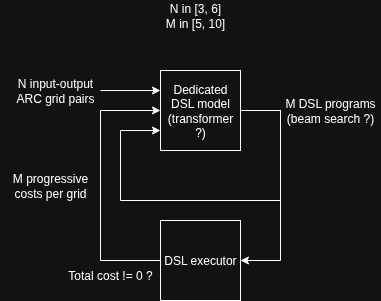
\includegraphics[width=0.82\linewidth]{diagram}}
\end{figure}

\subsection{Data Generation}
\label{sec:data}

We generate 10{,}000 valid DSL programs by random walks in the typed program
space, using the \texttt{TreeState} mask to guarantee syntactic validity.
For each program we compute its output on 3--6 randomly generated ARC grid pairs
(up to $30\times30$), producing the cost vector used for training.

\subsection{Inference: Iterative Cost-Guided Search}
\label{sec:inference}

Starting from the identity program \texttt{I}, the model iteratively:
(1)~encodes the current candidate programs and their costs;
(2)~proposes new programs via beam search (width 20);
(3)~executes proposed programs and computes actual costs;
(4)~retains the best $M=50$ candidates and repeats.

We observe that this process often follows a \textbf{star-shaped exploration
pattern}: the model tests multiple variations around a promising anchor program before
moving to a different region of the program space. This behavior provides a natural setting
for studying how the training regime interacts with search, since multiple partially explored
trajectories may coexist and contribute experience to subsequent model updates.

In addition to the search procedure itself, the training regime affects how experience is incorporated
into the model. We consider both synchronous and asynchronous training configurations. In the synchronous
setting, candidate generation and learning updates are organized around a single search trajectory, so
that successive variants of a candidate can be generated under a relatively stable model state. In the
asynchronous actor--learner setting, several search trajectories may be explored concurrently by actors
while a central learner continuously updates the model. Consequently, experiences generated from different
trajectories can be incorporated in an interleaved order: for example, candidates from trajectories $A$, $B$,
and $C$ may contribute to successive updates before later variants $A'$, $B'$, and $C'$ are processed.

This asynchronous organization exposes the model to a more interleaved stream of search experiences and allows
model updates to influence trajectories that are already in progress. The resulting interaction between exploration
and learning is therefore different from the more sequential exposure obtained in the synchronous setting.
We investigate whether this interleaving contributes to more effective navigation of the program space, in
particular by enabling experience acquired on one search trajectory to influence the exploration of others.

% ─────────────────────────────────────────────────────────────────────────────
\section{Experimental Setup}
\label{sec:setup}

\paragraph{Hardware.}
28 CPU cores for data generation and cost evaluation; one NVIDIA RTX~2000 GPU
for model training and inference.

\paragraph{Dataset.}
10{,}000 unique DSL programs with syntactic constraints, up to 128 tokens,
evaluated on grids up to $30\times30$.

\paragraph{Training.}
AdamW optimiser ($\mathrm{lr}=10^{-4}$), batch size of 1 task with $M=50$
candidate programs per iteration, online training over several hours.

\paragraph{Visualisation.}
Embeddings are extracted from the trained GNN encoder for 100 programs sorted by
length.
t-SNE (perplexity=30) and UMAP (cosine metric) projections are computed with
standard parameters.

% ─────────────────────────────────────────────────────────────────────────────
\section{Results}
\label{sec:results}

\subsection{Emergent Semantic Clustering}
\label{sec:clustering}

Both t-SNE (Fig.~\ref{fig:tsne}) and UMAP (Fig.~\ref{fig:umap}) projections
reveal a clearly structured latent space.
Rotations (\texttt{rot90}, \texttt{rot180}, \texttt{rot270}) form a dense,
well-separated cluster; mirrors occupy another distinct region; reductions are
grouped together; concatenations are separated by axis; and value transformations
lie in a transitional area.

Importantly, \textbf{no semantic label was provided during training}.
The structure emerged solely from the cost-guided objective and the DSL
type constraints.

\begin{figure}[htbp]
\floatconts
  {fig:tsne}
  {\caption{t-SNE visualisation of 10000 DSL program embeddings.
    Colour encodes the root primitive; point size encodes AST depth.
    Semantically related primitives cluster spontaneously.}}
  {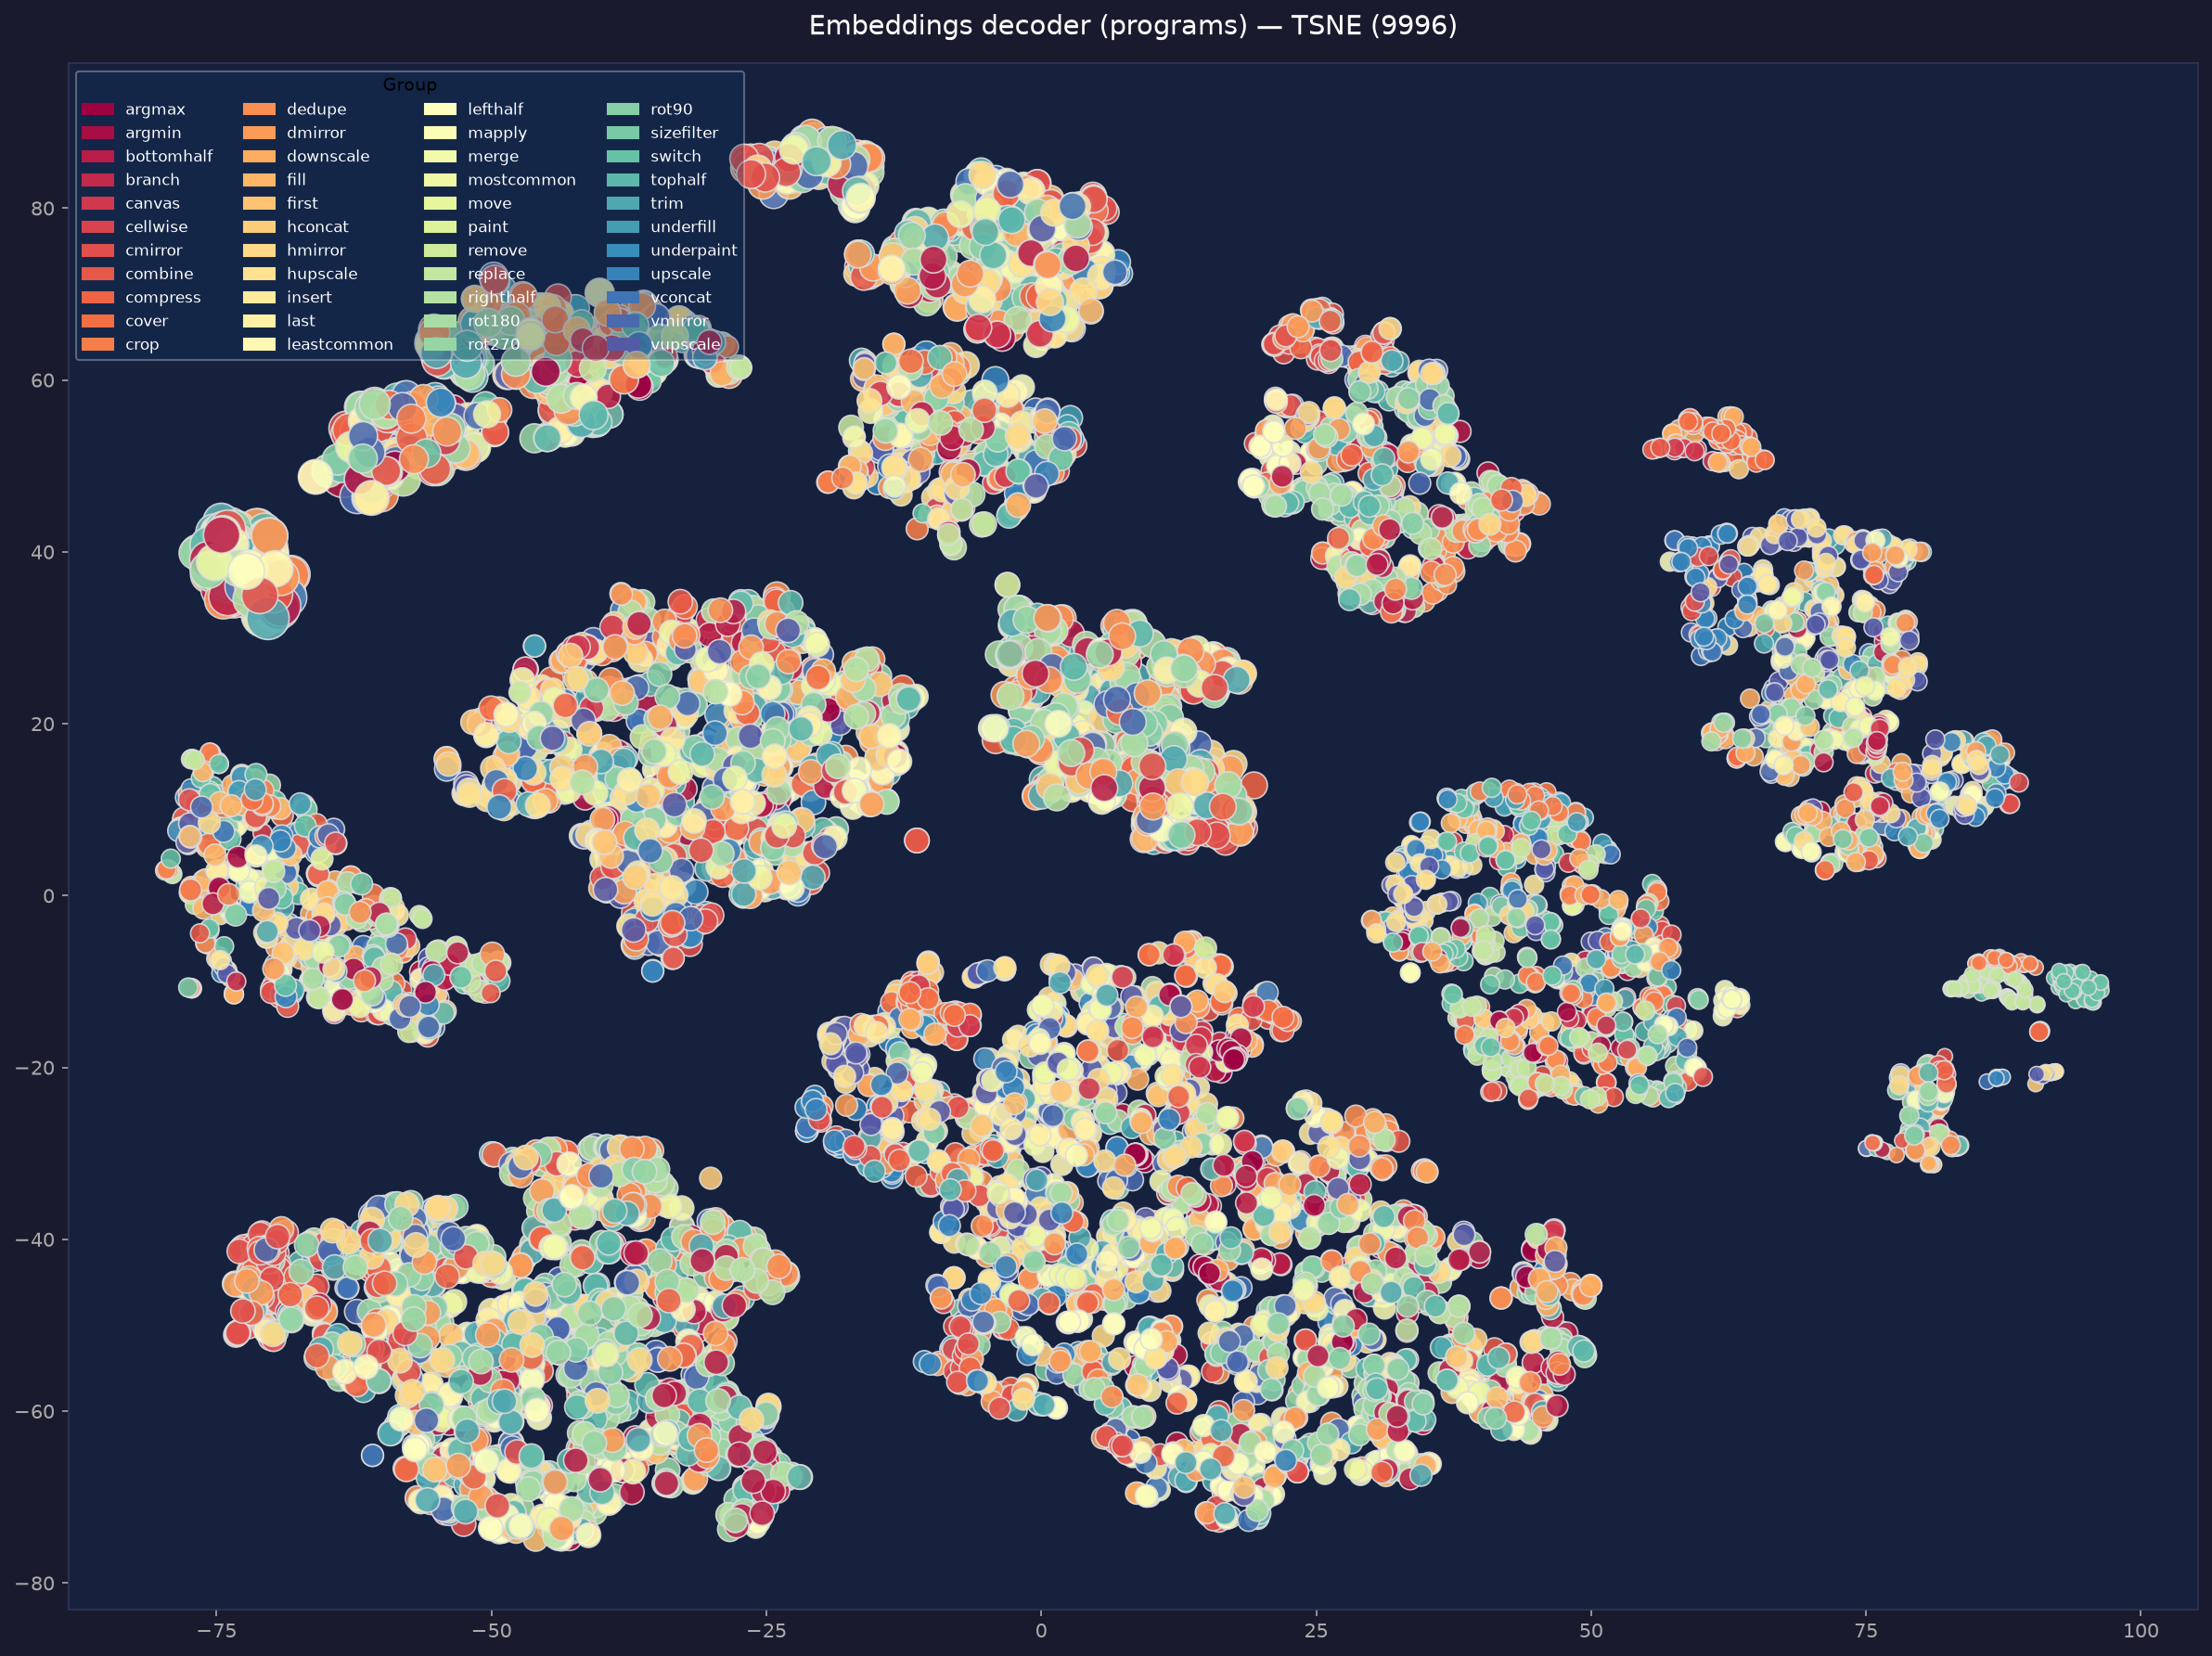
\includegraphics[width=\linewidth]{embeddings_tsne}}
\end{figure}

\begin{figure}[htbp]
\floatconts
  {fig:umap}
  {\caption{UMAP visualisation of 10000 DSL program embeddings.}}
  {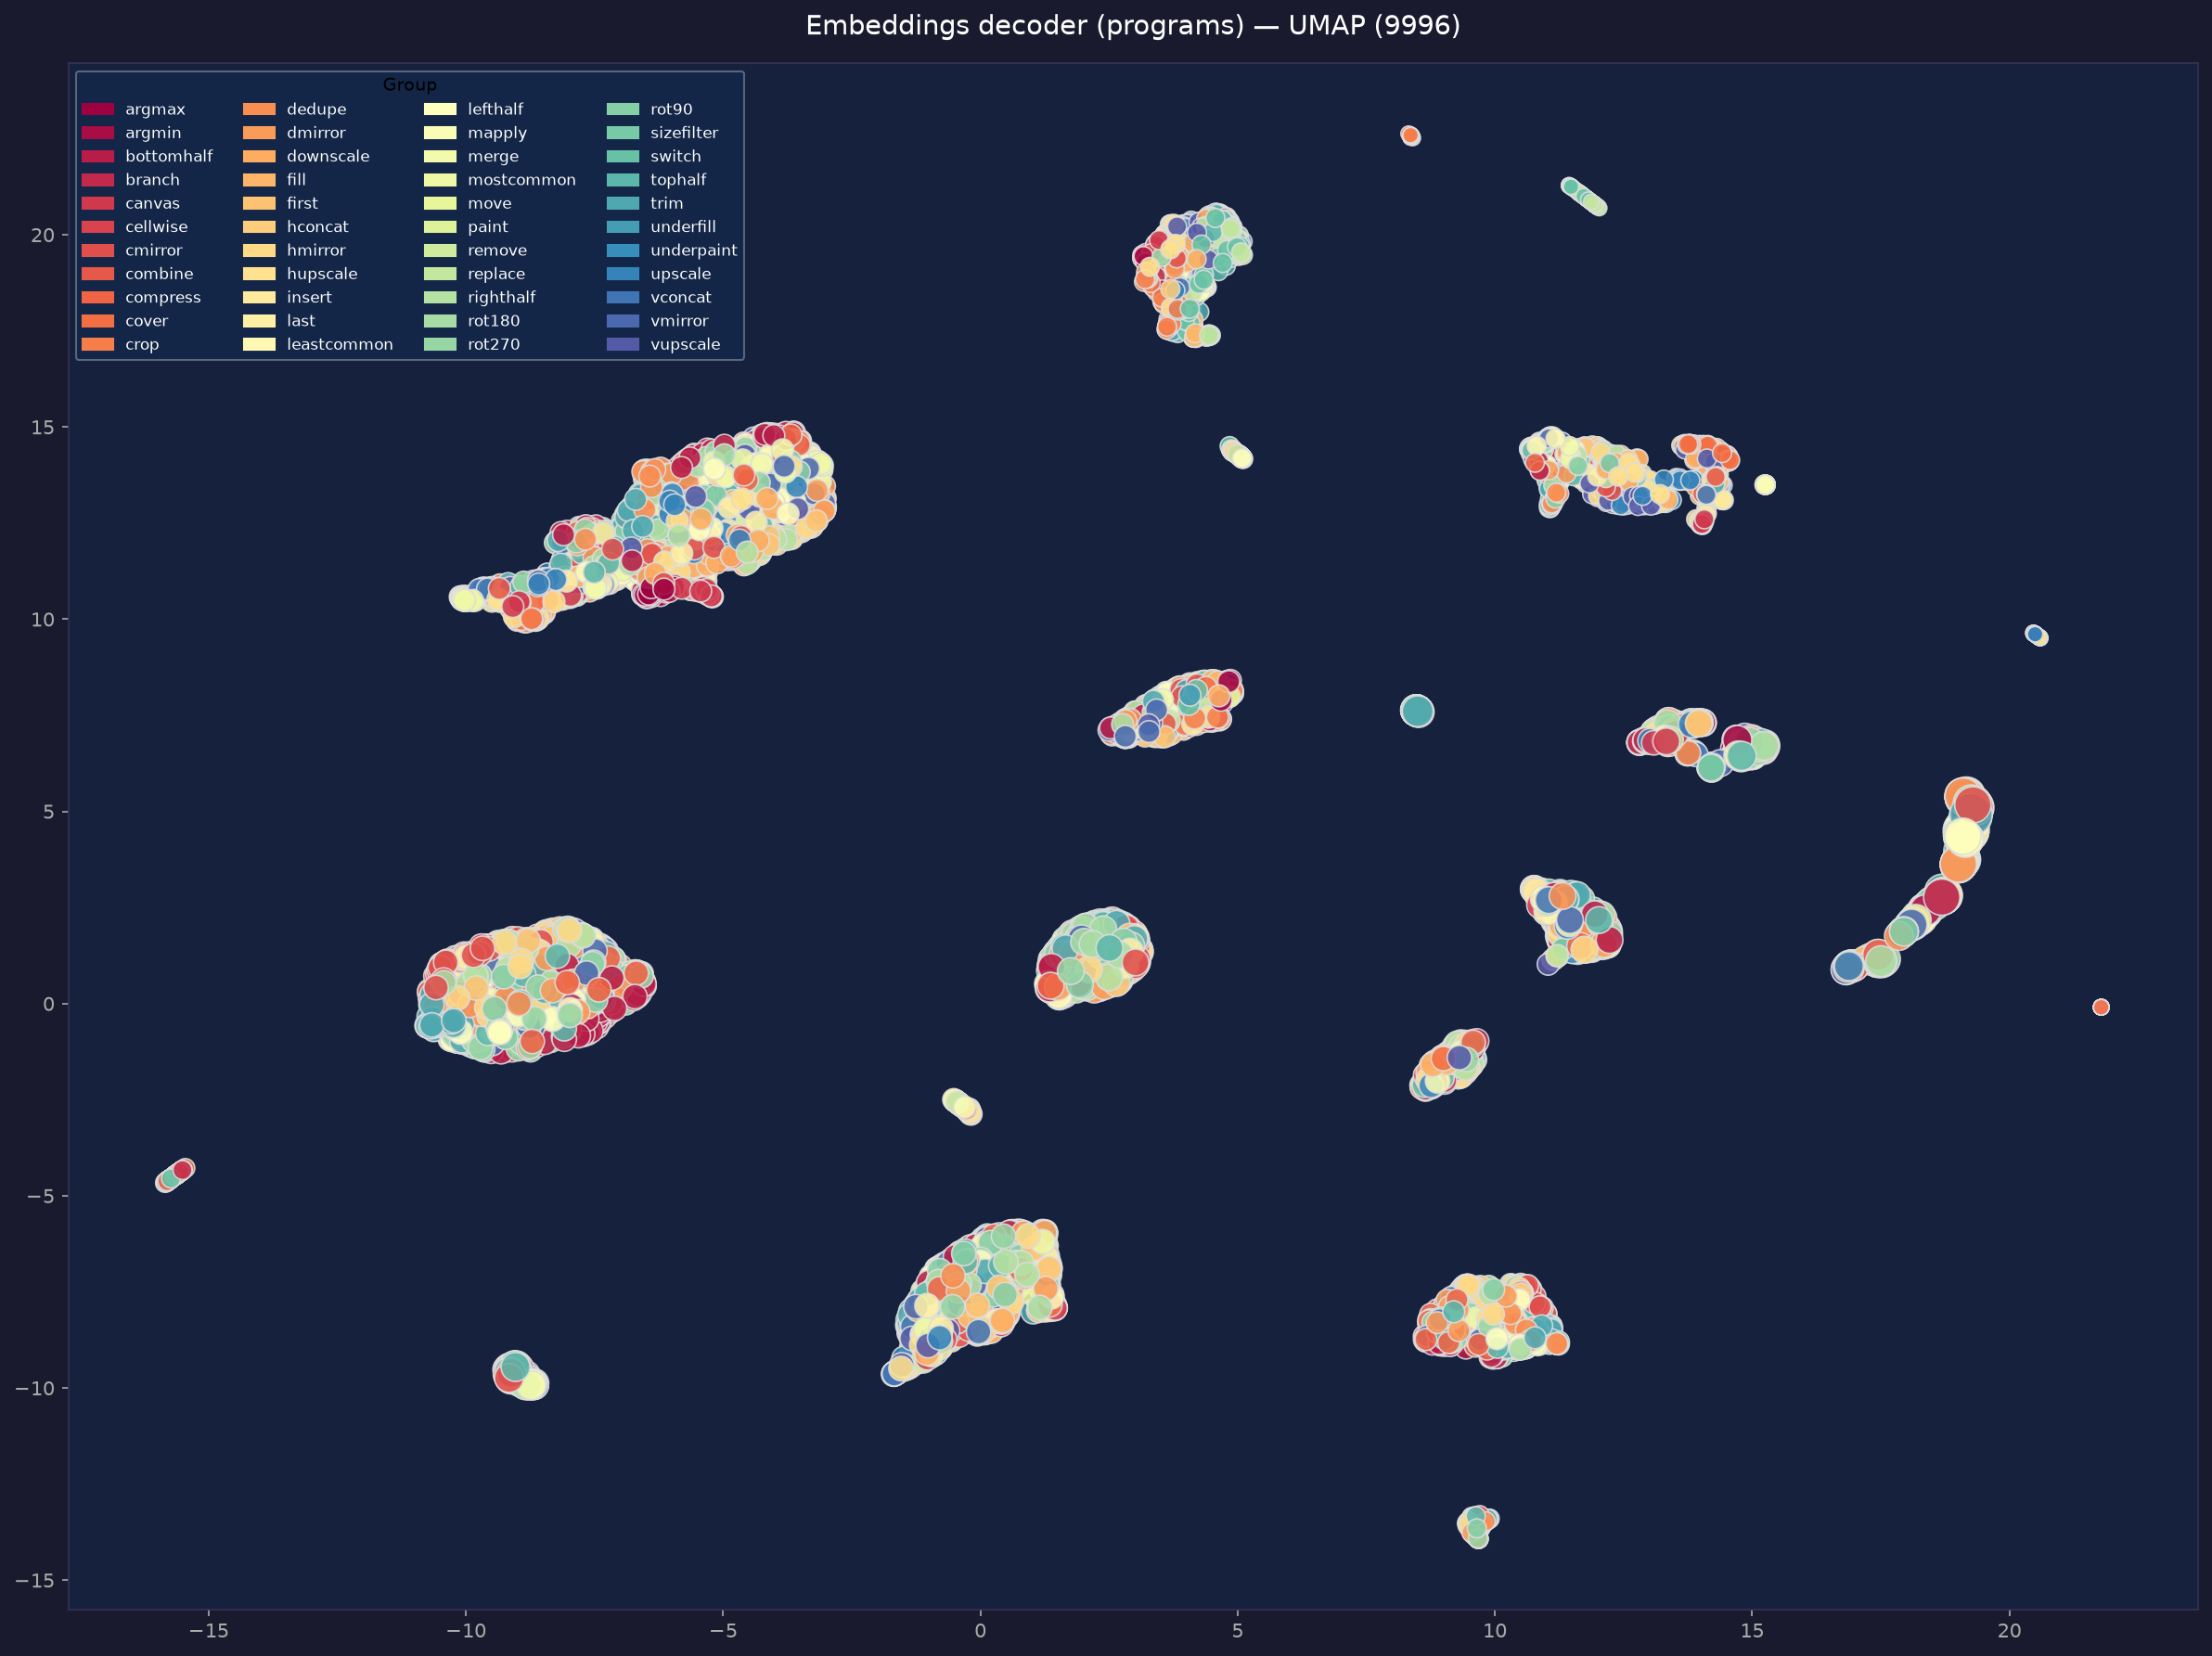
\includegraphics[width=\linewidth]{embeddings_umap}}
\end{figure}

\subsection{Compositionality and Continuity}
\label{sec:compositionality}

Programs composed of two primitives (e.g., \texttt{tophalf(trim(I))}) are
located midway between the clusters of their components, suggesting that the
embedding space is \textbf{compositional}: the vector of a composite program
approximates the sum of its parts.
Furthermore, a continuous path exists from \texttt{rot90(I)} to
\texttt{rot180(I)} to \texttt{rot270(I)}, indicating that the model learned a
smooth rotational manifold.

\subsection{Search Dynamics}
\label{sec:dynamics}

During iterative search, the model exhibits \textbf{anchor-based exploration}:
it first discovers a promising primitive (e.g., \texttt{tophalf(I)}), then
explores its neighbourhood systematically (e.g.,
\texttt{tophalf(rot90(I))}, \texttt{tophalf(vmirror(I))}), and finally jumps
to a better anchor.
An example trace is given in Appendix~\ref{apd:trace}.
This behaviour resembles \textbf{meta-cognition}: the model adapts its search
strategy based on observed progress.

\subsection{Comparison with LLM-based Baselines}
\label{sec:comparison}

Table~\ref{tab:comparison} compares our approach with four LLM baselines on the
ARC-AGI-2 training set using the same iterative pipeline.

\begin{table}[htbp]
\floatconts
  {tab:comparison}
  {\caption{Comparison of iterative DSL-synthesis approaches on
    ARC-AGI-2 training tasks (120 tasks evaluated).}}
  {%
  \begin{tabular}{lllll}
  \toprule
  \bfseries Model & \bfseries Architecture & \bfseries Resources
    & \bfseries Explainability & \bfseries Success (\%) \\
  \midrule
  GPT-5           & LLM (general)        & Cloud API       & Low  & 56.7 \\
  gpt-oss:120b    & LLM (open-weight)    & High-end GPU    & Low  & 31.7 \\
  \textbf{Ours}   & GNN+CNN+Transformer  & Local RTX~2000  & High & 10.8 \\
  llama3:8b       & LLM (open-weight)    & High-end GPU    & Low  & 0.0 \\
  mistral:7b      & LLM (open-weight)    & High-end GPU    & Low  & 0.0 \\
  \bottomrule
  \end{tabular}}
\end{table}

% ─────────────────────────────────────────────────────────────────────────────
\section{Discussion}
\label{sec:discussion}

\subsection{Why Does the Latent Space Self-Organise?}

We hypothesise that three factors are crucial.
First, the typed DSL with \texttt{TreeState} masking eliminates syntactically
invalid programs, removing noise from the learning signal.
Second, the multi-component cost function (size, bounding box, pixel overlap,
value) provides a rich, smooth gradient signal.
Third, training on \emph{improvement trajectories} -- rather than imitating a
fixed dataset -- encourages the model to learn a generalised notion of program
quality.

\subsection{Advantages over Existing Approaches}

Compared to LLM-based program synthesis, our approach (i)~is explicitly
constrained to produce only syntactically valid outputs; (ii)~provides
interpretable, visualisable embeddings; and (iii)~requires no massive
pre-training corpus.
Compared to pure symbolic search, it learns a distance metric over programs that
guides exploration and generalises across tasks.

\subsection{Limitations}

\textbf{Scalability.} Currently validated on grid transformations; extension to
other DSLs (e.g., Lean tactics) remains future work.
\textbf{Quantitative evaluation.} We evaluated the model on the public ARC-AGI-2 evaluation 
set as well as on the Kaggle ARC Prize competition leaderboard. In both cases, the success 
rate was 0\%, contrasting sharply with the 10.8\% recorded on the training set (the model being 
insufficiently trained).
\textbf{Generalization.} Whether the semantic map transfers to unseen task
distributions without fine-tuning requires further study.

% ─────────────────────────────────────────────────────────────────────────────
\section{Perspectives}
\label{sec:perspectives}

The results presented in this work suggest several directions for extending
the proposed approach beyond the ARC domain. A central property of the
architecture is the separation between the neural program-generation
mechanism and the domain-specific executable language. This separation makes
it possible to consider the definition of alternative DSLs for domains with
different structures, constraints, and objectives.

\subsection{Chess}
\label{subsec:perspectives-chess}

Chess provides a particularly interesting test case for this approach. A
chess-specific DSL could represent the state of a game as a typed board and
provide primitives corresponding to legal chess operations, such as selecting
a piece, computing its legal moves, moving a piece, capturing an opponent
piece, or performing special moves such as castling and en passant.

The resulting programs would represent explicit sequences of chess actions.
The symbolic execution engine could enforce the rules of the game and reject
illegal states or moves. The neural component could then learn to generate
structured sequences of legal operations rather than directly predicting
unconstrained board representations.

Such an extension would also make it possible to investigate whether the
proposed neural--symbolic interaction can learn increasingly long sequences
of dependent decisions. In contrast with ARC tasks, where a program generally
maps an input grid to an output grid, chess would introduce a dynamic state
space in which each operation modifies the state on which subsequent
operations depend.

\subsection{Computer-Aided Design}
\label{subsec:perspectives-cad}

Computer-aided design (CAD) represents another potential application domain.
A CAD-oriented DSL could expose geometric primitives and operations such as
creating points, lines, circles, surfaces, and solids, as well as operations
for translation, rotation, extrusion, intersection, subtraction, and
composition.

A generated program could therefore describe a construction procedure rather
than directly predicting the final geometry. The symbolic engine would
execute this procedure and produce the corresponding geometric object.

This approach could potentially provide an explicit and editable
representation of generated designs. In particular, the generated program
could be inspected, modified, or reused by a human designer. The same
principle could potentially apply to both two-dimensional and three-
dimensional CAD systems.

\subsection{Robotics}
\label{subsec:perspectives-robotics}

Robotics provides a further opportunity to investigate the combination of
neural generation and symbolic execution. A robotics DSL could represent
perception, spatial reasoning, planning, and actions through typed primitives.

For example, a program could combine operations for identifying an object,
computing a position, selecting a trajectory, and executing an action. The
symbolic component could enforce constraints on the available actions and
the state of the environment, while the neural component could propose
candidate action programs.

Such a representation could provide a natural interface between learned
decision-making and explicit task-level plans. The resulting programs could
also serve as interpretable descriptions of the actions selected by the
system.

\subsection{Autonomous Driving}
\label{subsec:perspectives-autonomous-driving}

A similar architecture could be considered for autonomous driving, provided
that the DSL is carefully designed around the safety and temporal constraints
of the domain.

A domain-specific language could represent operations such as identifying
objects, maintaining a representation of the surrounding environment,
evaluating possible trajectories, and selecting actions subject to explicit
constraints.
 
Rather than directly producing low-level control signals, a neural model
could generate structured decision programs that are subsequently validated
and executed by a symbolic component. This separation could make it possible
to inspect the intermediate decision process and to explicitly enforce
domain-specific constraints.

However, autonomous driving is substantially more safety-critical than the
domains considered in the present work. Such an application would therefore
require substantially stronger validation, formal guarantees, simulation, and
redundancy before deployment in a real system.

\subsection{Natural Language and Programmatic Reasoning}
\label{subsec:perspectives-language}

Natural language is another possible application domain. Instead of defining
a DSL directly over linguistic surface forms, the approach could employ a
domain-specific intermediate language whose primitives represent semantic
operations, transformations, or interactions with external tools.

The neural model could generate structured programs expressed in this
intermediate representation, while a symbolic interpreter would execute the
corresponding operations.

This perspective is particularly interesting because it provides a possible
bridge between natural-language interfaces and executable symbolic
representations. A natural-language instruction could be transformed into a
program whose individual operations remain explicit and independently
verifiable.

\subsection{A General Domain Adaptation Strategy}
\label{subsec:perspectives-generalization}

These examples suggest a general methodology for transferring the proposed
architecture to new domains. Let $\mathcal{D}$ denote a target domain and
let $\mathcal{L}_{\mathcal{D}}$ denote a DSL designed for that domain. The
adaptation process can be summarized as follows:

\begin{enumerate}
    \item define a vocabulary of domain-specific primitives;
    \item associate each primitive with explicit input and output types;
    \item provide executable semantics for each primitive;
    \item define a representation of programs suitable for neural processing;
    \item define an evaluation function for generated programs; and
    \item train the neural component to generate programs in
          $\mathcal{L}_{\mathcal{D}}$.
\end{enumerate}

The neural architecture can consequently remain largely independent of the
application domain, while the DSL and its execution engine provide the
domain-specific knowledge.

This separation is a central research question for future work. An important
objective would be to determine to what extent improvements to the general
program-generation mechanism transfer across domains, and to what extent
each new domain requires dedicated architectural or training modifications.

\subsection{Towards Composable Domain-Specific Intelligence}
\label{subsec:perspectives-composable}

A longer-term direction is to investigate whether several DSLs could be
combined into a hierarchy of increasingly general abstractions. A system
could, for example, combine geometric reasoning, physical interaction, and
high-level planning primitives in a robotics setting.

Such a hierarchy would make it possible to investigate whether a neural model
can learn to compose heterogeneous symbolic operations while relying on the
execution engine to maintain domain-specific constraints.

More generally, this suggests viewing the DSL not merely as a restricted
programming language, but as an explicit interface between learned models and
executable domain knowledge.

% ─────────────────────────────────────────────────────────────────────────────
\section{Conclusion}
\label{sec:conclusion}

We have presented a neuro-symbolic architecture for program synthesis that learns
a semantic latent space of DSL programs purely from a cost-guided objective.
The resulting embeddings self-organise into interpretable clusters without any
explicit semantic labels, and the inference procedure exhibits emergent
meta-cognitive search strategies.

These results suggest that typed DSLs combined with multi-component cost
functions and iterative online training offer a promising path toward
\textbf{explainable, data-efficient program synthesis} -- addressing two of the
most under-explored areas in neuro-symbolic AI: explainability and meta-cognition.

\acks{The author thanks the open-source community for providing PyTorch, PyTorch
Geometric, and scikit-learn. This research received no specific funding.}

\bibliography{nesy2027-livet}

% ─────────────────────────────────────────────────────────────────────────────
\appendix

\section{Hyperparameters}
\label{apd:hyper}

\begin{table}[htbp]
\floatconts
  {tab:hyper}
  {\caption{Model hyperparameters.}}
  {%
  \begin{tabular}{lll}
  \toprule
  \bfseries Component & \bfseries Parameter & \bfseries Value \\
  \midrule
  GNN         & layers             & 3 \\
  GNN         & hidden dim         & 128 \\
  CNN         & layers             & 4 \\
  CNN         & channels           & 64$\to$64$\to$128$\to$128 \\
  Transformer & decoder layers     & 4 \\
  Transformer & $d_{\mathrm{model}}$ & 256 \\
  Transformer & heads              & 8 \\
  Training    & learning rate      & $10^{-4}$ \\
  Inference   & beam width         & 20 \\
  Inference   & max program length & 128 tokens \\
  \bottomrule
  \end{tabular}}
\end{table}

\section{Example Search Trace}

\subsection{Extract of dsl\_model.md}
\label{apd:trace}

The following trace illustrates the iterative cost-guided search.

\begin{markdown}
# 1/961 Target program: `trim(I)` (trajectory: 93 programs)
- 2026-08-26 09:58:32.355692 #0(0)/1 Searched program (1/93): `switch(I, ONE, TWO)`, cost: `3338.632368475567`
    - Program pool
        - Program: `I`, cost: `3350.632368475567`
        - Program: `I`, cost: `3350.632368475567`
        - Program: `I`, cost: `3350.632368475567`
        - Program: `I`, cost: `3350.632368475567`
        - Program: `I`, cost: `3350.632368475567`
        - Program: `I`, cost: `3350.632368475567`
        - Program: `I`, cost: `3350.632368475567`
        - Program: `I`, cost: `3350.632368475567`
        - Program: `I`, cost: `3350.632368475567`
        - Program: `I`, cost: `3350.632368475567`
    - **Found worst program:** `vmirror(I)`, cost: `3350.632368475567`
    - **Found worst program:** `lefthalf(I)`, cost: `3393.2498693133093`
    - **Found worst program:** `rot270(I)`, cost: `3377.604177212805`
    - **Found worst program:** `hmirror(I)`, cost: `3350.632368475567`
    - **Found worst program:** `dedupe(I)`, cost: `3350.632368475567`
    - **Found worst program:** `cmirror(I)`, cost: `3377.604177212805`
    - **Found worst program:** `compress(I)`, cost: `3350.632368475567`
    - **Found worst program:** `branch(T, I, I)`, cost: `3350.632368475567`
    - **Found worst program:** `dmirror(I)`, cost: `3377.604177212805`
    - **Found worst program:** `righthalf(I)`, cost: `3430.2498693133093`
    - **Found worst program:** `vconcat(I, I)`, cost: `10004.2107936166`
    - *Found better program:* `trim(I)`, cost: `0.0`
Found program: `trim(I)` (16(12)/95 iterations)
# 2/961 Target program: `rot90(I)` (trajectory: 108 programs)
- 2026-08-26 09:58:33.619647 #0(0)/1 Searched program (1/108): `vconcat(cmirror(I), canvas(SEVEN, increment(UP)))`, cost: `2568.1364918359345`
    - Program pool
        - Program: `I`, cost: `2576.6696437031455`
        - Program: `I`, cost: `2576.6696437031455`
        - Program: `I`, cost: `2576.6696437031455`
        - Program: `I`, cost: `2576.6696437031455`
        - Program: `I`, cost: `2576.6696437031455`
        - Program: `I`, cost: `2576.6696437031455`
        - Program: `I`, cost: `2576.6696437031455`
        - Program: `I`, cost: `2576.6696437031455`
        - Program: `I`, cost: `2576.6696437031455`
        - Program: `I`, cost: `2576.6696437031455`
    - **Found worst program:** `crop(hmirror(hmirror(I)), UNITY, UP)`, cost: `6355.92407534942`
    - **Found worst program:** `hmirror(hmirror(dedupe(I)))`, cost: `5108.635176843368`
    - **Found worst program:** `crop(hmirror(dedupe(I)), ORIGIN, UP)`, cost: `6355.92407534942`
    - **Found worst program:** `crop(hmirror(hmirror(I)), toivec(TWO), UNITY)`, cost: `6339.986342171008`
    - **Found worst program:** `hmirror(switch(lefthalf(I), decrement(ONE), ONE))`, cost: `4290.497533825093`
    - **Found worst program:** `switch(hmirror(hmirror(I)), TWO, ONE)`, cost: `2680.6696437031455`
    - *Found better program:* `rot270(hmirror(vmirror(I)))`, cost: `0.0`
Found program: `rot270(hmirror(vmirror(I)))` (8(7)/52 iterations)
# 3/961 Target program: `dedupe(I)` (trajectory: 563 programs)
- 2026-08-26 09:58:34.388240 #0(0)/1 Searched program (1/563): `cover(rot270(I), dneighbors(lrcorner(neighbors(UP))))`, cost: `2672.8400280289097`
    - Program pool
        - Program: `I`, cost: `2697.4256661510863`
        - Program: `I`, cost: `2697.4256661510863`
        - Program: `I`, cost: `2697.4256661510863`
        - Program: `I`, cost: `2697.4256661510863`
        - Program: `I`, cost: `2697.4256661510863`
        - Program: `I`, cost: `2697.4256661510863`
        - Program: `I`, cost: `2697.4256661510863`
        - Program: `I`, cost: `2697.4256661510863`
        - Program: `I`, cost: `2697.4256661510863`
        - Program: `I`, cost: `2697.4256661510863`
    - *Found better program:* `crop(hmirror(hmirror(hmirror(I))), UNITY, UNITY)`, cost: `1411.3630833845389`
- 2026-08-26 09:58:34.438827 #1(1)/2 Searched program (373/563): `crop(I, UNITY, UP)`, cost: `1411.293765408777`
    - Program pool
        - Program: `I`, cost: `2697.4256661510863`
        - Program: `I`, cost: `2697.4256661510863`
        - Program: `I`, cost: `2697.4256661510863`
        - Program: `I`, cost: `2697.4256661510863`
        - Program: `I`, cost: `2697.4256661510863`
        - Program: `I`, cost: `2697.4256661510863`
        - Program: `I`, cost: `2697.4256661510863`
        - Program: `I`, cost: `2697.4256661510863`
        - Program: `I`, cost: `2697.4256661510863`
        - Program: `crop(hmirror(hmirror(hmirror(I))), UNITY, UNITY)`, cost: `1411.3630833845389`
    - **Found worst program:** `dmirror(I)`, cost: `2707.8400280289097`
    - **Found worst program:** `cmirror(I)`, cost: `2707.8400280289097`
    - *Found better program:* `dedupe(I)`, cost: `0.0`
\end{markdown}

\subsection{GPT-5}
\label{apd:gpt5}

\textbf{Input prompt:} \url{https://github.com/Julien-Livet/aicpp/blob/dev/scripts/data/gpt/gpt-5/training/1caeab9d-input-002.md}

\textbf{Output:} \url{https://github.com/Julien-Livet/aicpp/blob/dev/scripts/data/gpt/gpt-5/training/1caeab9d-output-002.md}

\subsection{gpt-oss:120b}
\label{apd:gpt-oss}

\textbf{Input prompt:} \url{https://github.com/Julien-Livet/aicpp/blob/dev/scripts/data/ollama/gpt-oss_120b-cloud/training/1caeab9d-input-005.md}

\textbf{Output:} \url{https://github.com/Julien-Livet/aicpp/blob/dev/scripts/data/ollama/gpt-oss_120b-cloud/training/1caeab9d-output-005.md}

\end{document}
